\documentclass[border=5mm]{standalone}
\usepackage{tikz}
\usepackage{tikz-qtree}

\begin{document}
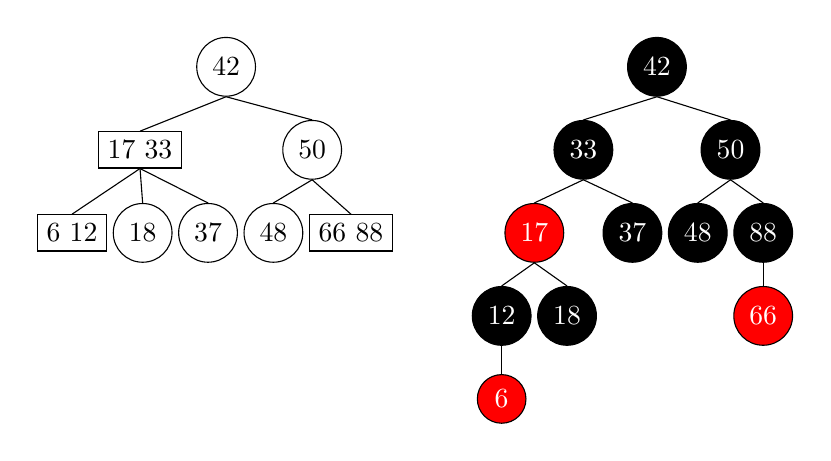
\begin{tikzpicture}[every tree node/.style={align=center}]
    \matrix[row sep=1cm, column sep=1cm] {
    \Tree
    [.\node[draw, circle]{42};
    [.\node[draw, rectangle]{17 33};
    [.\node[draw, rectangle]{6 12}; ]
    [.\node[draw, circle]{18}; ]
    [.\node[draw, circle]{37}; ]
    ]
    [.\node[draw, circle]{50};
    [.\node[draw, circle]{48}; ]
    [.\node[draw, rectangle]{66 88}; ]
    ]
    ];
    &
    \Tree
    [.\node[draw, fill=black, circle]{\textcolor{white}{42}};
    [.\node[draw, fill=black, circle]{\textcolor{white}{33}};
    [.\node[draw, fill=red, circle]{\textcolor{white}{17}};
    [.\node[draw, fill=black, circle]{\textcolor{white}{12}};
    [.\node[draw, fill=red, circle]{\textcolor{white}{6}}; ]
    ]
    [.\node[draw, fill=black, circle]{\textcolor{white}{18}}; ]
    ]
    [.\node[draw, fill=black, circle]{\textcolor{white}{37}}; ]
    ]
    [.\node[draw, fill=black, circle]{\textcolor{white}{50}};
    [.\node[draw, fill=black, circle]{\textcolor{white}{48}}; ]
    [.\node[draw, fill=black, circle]{\textcolor{white}{88}};
    [.\node[draw, fill=red, circle]{\textcolor{white}{66}}; ]
    ]
    ]
    ]; \\
    };
\end{tikzpicture}
\end{document}
